\section{Introduction}

A growing body of research literature uses trait-based approaches to understand how biodiversity links to ecosystem functioning, and how environmental changes are likely to affect species non-randomly with respect to their traits (Hevia et al). Strictly, traits are defined as characteristics measurable the level of an individual, with an effect on organismal fitness or performance. They can be physiological (e.g., metabolic rates), morphological (e.g., body mass), behavioural (e.g., learning) or phenological (e.g., anthesis), or can relate to species life-history (e.g. longevity). This definition can be broadened to include characteristics measurable at the species level, such as the number of habitats known to be used by a species (habitat breadth). I broaden the strict definition of traits to include such other ecological characteristics, and I refer to these as ecological traits.

Many studies have shown that traits influence species responses to environmental pressures (). Moreover, it is now accepted that ecosystem functioning is positively correlated with species functional diversity. Species traits can provide a mechanistic understanding of both species roles in ecosystem functioning and of species responses to changes. Traits shape species fundamental and realised niches; for instance, physiological traits influence species thermal tolerances, participating in defining their geographical distributions. Traits such as trophic level or body mass structure food webs and affect inter- and intra-specific competition. As such, traits determine and reflect species use of their environment. Specifically, effect traits define organismal contributions to ecosystem functions. Effect traits are underpinned by species resource use, and this applies at diverse scales, from single-celled nutrient cycling bacteria to large mammals. Response traits are those involved in determining species responses to environmental changes and can overlap with effect traits. 

Although terrestrial vertebrates have been extensively studied in the past (Titley et al), the vast majority of research investigating the impact of environmental changes on ecosystem functions has focused on plants and invertebrates (Hevia et al). Vertebrates nevertheless play diverse ecosystem roles, and some are important keystone species.  Vertebrate species particularly contribute in food web structures and population dynamics through predatory and herbivory activity. They are pollinators and seed dispersers, and overall participate in nutrient cycling at higher levels. Understanding how environmental changes may affect their ecological roles is important to predict future ecosystem functioning, and to put into place appropriate mitigation measures. The end-goals of my PhD thesis are to elucidate how species traits influence their responses to land-use and climate change, and how this links to changes in ecosystem functioning. Addressing these questions requires to use extensive trait data.  Despite vertebrates having been the focus of much research, and despite the growing interest for trait-based approaches, there exist no comprehensive database of vertebrate ecological traits encompassing all classes. Consequently, collating trait data is a prerequisite for any further work, and this operation is constrained by the amount of information available in the literature. Thanks to past and recent effort to release data in the public domain, at least four comprehensive ecological trait databases have been published (mammals: Pantheria, amphibians: Amphibio, amniotes: Myhrvold, mammals and birds: Cooke et al). Other traits have been made available through online platforms alongside published articles (e.g. GARD), or can be downloaded from online databases (IUCN Redlist, Birdzone). Trait data for mammals and birds is likely to be more abundant and more resolved than for reptiles and amphibians, due to systematic biases in sampling with regards to taxonomic groups (Newbold, manuscript).
 
I collected ecological trait information for terrestrial vertebrates from diverse primary sources. Trait selection was motivated by two main reasons: (1) traits should be of ecological interest and be related to response of effect processes; (2) trait values should be available for many species, across the four terrestrial vertebrate classes, allowing for cross-classes comparative analyses. Selected targeted traits related to species life-history and morphology (body mass; longevity; litter/clutch size; diel activity; trophic level; diet) and to their habitat preferences (habitat breadth and specialisation). Reptilian diet was not readily available in primary data sources, and one exception was made as I extracted the data for the other classes.

% detail ecological relevance of traits

The present chapter details the methodology employed to collate trait information. I elaborate on some of the challenges met when compiling data across many species, such as inconsistency of taxonomy across sources. Not unexpectedly, the amount of missing values was highly variable across classes and traits. To achieve full coverage, I imputed missing trait values using random-forest algorithms. Here, I briefly examine imputation robustness by looking at whether results from several imputations were congruent. 

In October 2018, Cooke et al released a database of six mammalian and avian traits, using similar primary sources. They collated and imputed missing trait values for body mass, litter/clutch size, volancy, diel activity, primary diet and habitat breadth. I did not use their collected data for two reasons: first, similar primary sources were used in both our compilations; second, they used different missing data imputations methods. I used this freely accessible data as an opportunity to compare the results of both our data collection and imputation process. This chapter also presents the results of this comparison.

% Finally, I discuss the weaknesses of the methodology
% Impossibility to get intra-specific variation.


\pagebreak
\section{Methods}

\subsection{Ecological trait data collection}

\subsubsection{Primary data sources.}
I collated ecological trait data for terrestrial vertebrates from the sources figuring in Table \ref{datasources}. Information was compiled for the following target traits: body mass, longevity, litter or clutch size, trophic level, diel activity, diet, and habitat preferences. I also compiled traits that were potentially correlated to either body mass or longevity, to be used as potential predictors in imputations of missing values. As such, body length information was compiled when available, as well as generation length or age at sexual maturity. Most notably, longevity was chosen over generation length or age at sexual maturity as it was the only common currency across classes reflecting generation turnover. In addition, species geographical range sizes were calculated from distribution data, extracted from the IUCN Red List.

% TO REVIIIIIISE
% Table of sources.
\begin{table}[h!]
\renewcommand{\baselinestretch}{1}
\renewcommand{\arraystretch}{1.5}
\begin{center}\fontsize{9}{11}\selectfont
\caption[Data sources for trait compilation]{\textbf{Data sources for trait compilation.} I here show were I extracted trait data from for each class. These individual sources may more traits than shown here. BM: body mass; BL: body length; L: longevity or maximum longevity; GL: generation length; LCS: litter or clutch size; TL: trophic level; Di: diet; DA: diel activity; RS: range size; H: habitat data. Target traits are bolded; other traits were added for potential correlations in further imputations.} 
\label{datasources}
\begin{tabular}{|l|c|c|c|c|c|c|c|c|c|c|c|c|}
\hline
\multicolumn{1}{|c|}{\multirow{2}{*}{\textbf{Sources}}} & \multirow{2}{*}{\textbf{Taxa}} & \multicolumn{9}{c|}{\textbf{Traits}} & \multirow{2}{*}{\textbf{RS}} & \multirow{2}{*}{\textbf{H}} \\ \cline{3-11}
\multicolumn{1}{|c|}{} &  & \textbf{BM} & BL & \textbf{L} & MA & GL & \textbf{LCS} & \textbf{TL} & \textbf{Di} & \textbf{DA} &  &  \\ \hline
Amphibio & \multirow{4}{*}{Amphibians} & \checkmark & \checkmark & \checkmark & \checkmark &  & \checkmark &  & \checkmark & \checkmark &  &  \\ \cline{1-1} \cline{3-13} 
Cooper &  &  & \checkmark &  &  &  & \checkmark &  &  &  & \checkmark &  \\ \cline{1-1} \cline{3-13} 
Senior &  &  & \checkmark &  &  &  &  &  &  &  &  &  \\ \cline{1-1} \cline{3-13} 
Bickford &  &  & \checkmark &  &  &  &  &  &  &  & \checkmark &  \\ \hline
Elton & \multirow{2}{*}{Birds} & \checkmark &  &  &  &  &  &  & \checkmark & \checkmark &  &  \\ \cline{1-1} \cline{3-13} 
Butchart &  & \checkmark &  & \checkmark &  &  &  &  &  &  &  &  \\ \hline
Pantheria & \multirow{5}{*}{Mammals} & \checkmark & \checkmark & \checkmark & \checkmark &  & \checkmark & \checkmark &  & \checkmark &  &  \\ \cline{1-1} \cline{3-13} 
Kissling1 &  &  &  &  &  &  &  & \checkmark & \checkmark &  &  &  \\ \cline{1-1} \cline{3-13} 
Kissling2 &  &  &  &  &  &  &  & \checkmark & \checkmark &  &  &  \\ \cline{1-1} \cline{3-13} 
Elton &  & \checkmark &  &  &  &  &  &  & \checkmark & \checkmark &  &  \\ \cline{1-1} \cline{3-13} 
Pacifici &  & \checkmark &  & \checkmark & \checkmark & \checkmark &  &  &  &  &  &  \\ \hline
Scharf & \multirow{8}{*}{Reptiles} & \checkmark &  & \checkmark & \checkmark &  & \checkmark & \checkmark &  & \checkmark &  &  \\ \cline{1-1} \cline{3-13} 
Meiri &  &  &  &  &  &  &  & \checkmark &  & \checkmark &  &  \\ \cline{1-1} \cline{3-13} 
Vidan &  &  &  &  &  &  &  &  &  & \checkmark &  &  \\ \cline{1-1} \cline{3-13} 
Stark &  & \checkmark &  & \checkmark &  &  & \checkmark &  &  & \checkmark &  &  \\ \cline{1-1} \cline{3-13} 
Schwarz &  &  &  &  &  &  & \checkmark &  &  &  &  &  \\ \cline{1-1} \cline{3-13} 
Novosolov1 &  & \checkmark &  &  &  &  &  & \checkmark &  &  & \checkmark &  \\ \cline{1-1} \cline{3-13} 
Novosolov2 &  &  &  &  &  &  & \checkmark &  &  &  &  &  \\ \cline{1-1} \cline{3-13} 
Slavenko &  & \checkmark &  &  &  &  &  &  &  &  &  &  \\ \hline
Myhrvold & Amniotes & \checkmark & \checkmark & \checkmark & \checkmark &  & \checkmark &  &  &  &  &  \\ \hline
IUCN & Vertebrates &  &  &  &  &  &  &  &  &  & \checkmark & \checkmark \\ \hline
\end{tabular}
\end{center}
\end{table}

\subsubsection{Compilation methods.}

\paragraph{Continuous traits.}
All continuous traits were averaged within species when different sources provided estimates. Longevity and maximum longevity were assumed to provide the same information and were averaged within species. No measure of intra-specific variability was compiled and estimates were provided as a single measure for each species.

\paragraph{Categorical traits.}
\subparagraph{Diet and diet breadth.} Even though diet was not available from any primary source for reptiles, I compiled diet information for all other classes. Species diet was described in primary sources as a binary variable recording whether food items were known to be consumed by a species or not. I calculated diet breadth as the number of food items a species was recorded to ingest. In addition,  species were pooled into 5 categories in one of the source (Elton birds) according to their primary diet (food items that constituted more than 50\% of the species diet). I adopted the same system and  pooled species into the 5 following primary diet categories: (1) seed or plant consumers; (2) fruit or nectar consumers; (3) invertebrate consumers; (4) vertebrate consumers (including scavengers); (5) omnivores. More details on diet compilation are provided in the SI. 
\subparagraph{Trophic level.} For amphibians and birds, trophic levels were partly inferred from the primary diet. 
\subparagraph{Habitat preferences.}
Species habitat preferences were compiled from IUCN habitat data files and were described as a binary variable recording whether a species was known to occur in a particular habitat. I calculated habitat breadth as the number of habitats a species was known to use. Weights were assigned to each habitat in this calculation depending on the recorded habitat suitability and importance; outcomes were not sensitive to different weight choices (SI). Finally, a broad degree of habitat specialisation was produced. If any artificial habitat was recorded to be suitable, species were reported to be generalists; else, they were natural habitat specialists. More details on habitat preferences compilation are provided in the SI. 

\subsection{Phylogenetic information}
I obtained phylogenetic trees for birds, amphibians, mammals and squamates from Hedges et al (2015), (available at http://www.biodiversitycenter.org/ttol, downloaded 06/07/2018).

\subsection{Tackling taxonomic synonymy}

Across the different primary sources, similar species could appear under different binomial names. This was a problem when matching datasets by species. It was also problem when matching species to the PREDICTS database. Moreover, it is possible than within a primary source, a given species was appearing under two or more different names. As such, taxonomic synonymy created `pseudoreplicates' of the same species, overall falsely increasing the total number of species and artificially inflating the amount of missing trait values. Taxonomic synonymy was hence a major issue; due to the large number of species across datasets, extensive manual checks could not be applied. The presence of typos in species names had the same effect as synonymy, erroneously duplicating species. I attempted to correct for taxonomy first by correcting for typos, and second by identifying species which were entered under a synonymic name and replacing these with the accepted name. To this end, I developed an automated procedure, complemented with a few manual entries. Obvious cases where vernacular names had been entered in the place of binomial names were also treated manually; that was the case for 44 PREDICTS species (when possible, I best assigned binomial names to species common names; unidentifiable species were left empty and assigned to a genus (5 species)).

\subsubsection{Automated procedure and outputs.}
\paragraph{Extracting names from the RedList and the Integrated Taxonomic Information System (ITIS).}
The automated procedure consisted in extracting species accepted and synonymic binomial names from the IUCN Red List or from the ITIS, using the rredlist and taxize R packages. I started by generating a list of all names figuring across datasets (primary sources, phylogenies and PREDICTS). These `original' names were corrected for typos; then, the IUCN RedList was queried and synonyms and accepted names were stored when possible. When species were not found in the IUCN Red List, information was extracted from ITIS. When species were not found in ITIS either, corrected names were assumed to be accepted. Family and order information was extracted using the same procedure and some entries were completed using the Global Biodiversity Information Facility taxonomic backbone (https://www.gbif.org/tools/species-lookup).\\
\textbf{NB:} for species entered with the forms \textit{Genus cf.}, \textit{Genus aff.} or \textit{Genus spp.}, the accepted name was left empty.An extra column indicates whether the species is known only at the genus level.

\paragraph{Outputs.} I generated a dataset of vertebrate species names found across datasets, recording whether names were accepted or synonymic. For each name, the accepted name and the synonyms were stored, as well as additional taxonomic information (order, family, genus).

\paragraph{Harmonising taxonomy in trait datasets.}
Taxonomy across datasets was finally homogenised by replacing recorded synonyms with their accepted scientific names. Overall, this procedure  reduced the total number of species figuring in trait datasets (Figure \ref{taxcor}). The species presenting the highest degree of pseudoreplication was the East African mole rat (\textit{Tachyoryctes splendens}), which was figuring under 12 different names across primary sources (Figure \ref{taxcor}B).

% figure: distribution of names and differences in species number
\vspace{0.5cm}
\begin{figure}[h!]
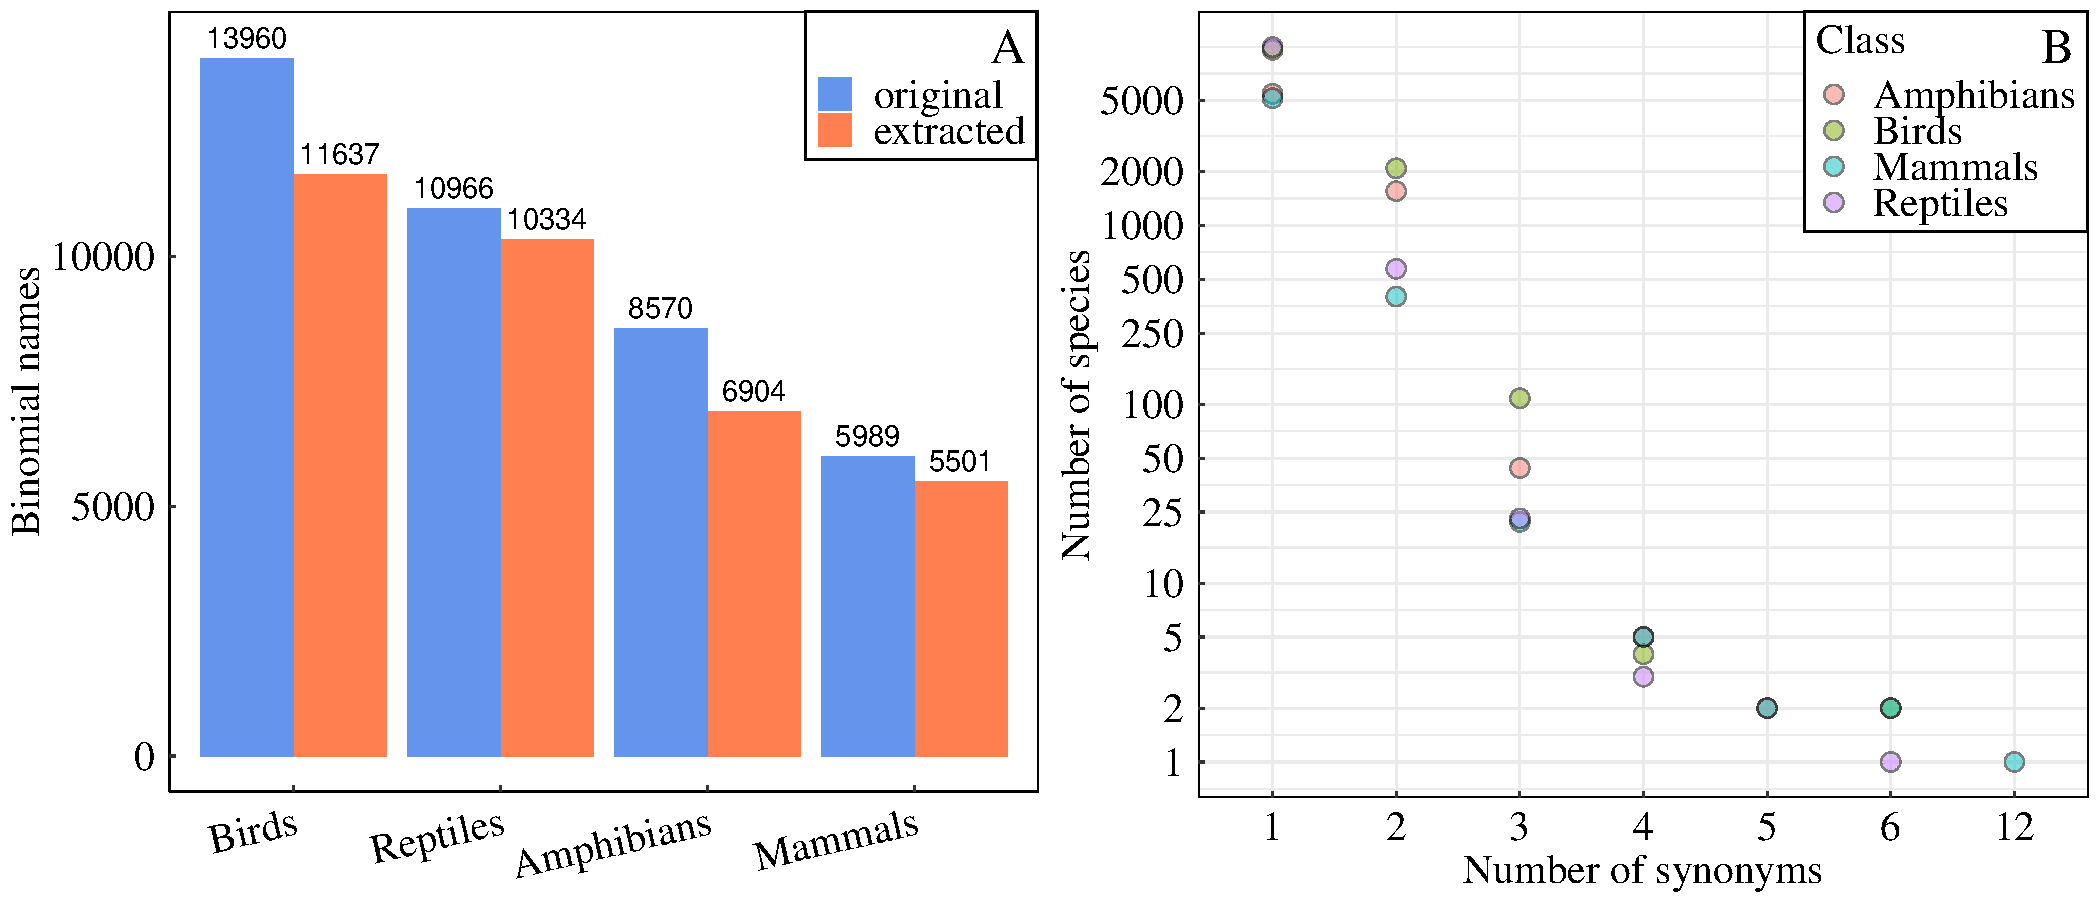
\includegraphics[scale=0.45]{figures/chapter2/Taxonomic_corrections/tax_corrections}
\caption[Difference in species number due to taxonomic correction (A) and distribution of number of synonyms across datasets (B)]{\textbf{Difference in species number due to taxonomic correction (A) and distribution of number of synonyms across datasets (B).} \textbf{(A)} shows the number of species across all primary sources (trait datasets, PREDICTS, phylogenies), before and after correcting for taxonomy. Replacing identified synonyms by the extracted accepted name reduced the number of species in all classes, with the most drastic reduction for birds (decrease by 2,323 unique binomial names). The diminution was of 632 unique identified species for reptiles, of 1,666 for amphibians and of 488 for mammals. \textbf{(B)} shows the distribution of the number of synonymic names. In all four classes, more than 5,000 species (or binomial names) had no identified synonyms. Nevertheless, a large amount of species had two identified synonyms (range: 400 species for mammals - 2086 for birds). The most replicated species was the East African mole rat \textit{Tachyoryctes splendens}, for which 11 synonyms were identified.}
\label{taxcor}
\end{figure}

Despite the automation efforts, taxonomic redundancy persisted in the trait datasets. Indeed, at this stage, not all species in PREDICTS matched a species in the trait datasets. Additional manual inputs were required to resolve taxonomic synonymy for these species. Verifying the presence of PREDICTS species in trait datasets was important for further analyses. Taxonomic synonymy was resolved manually for 91 PREDICTS species that did not match any species in the trait datasets; in that case, information was extracted from other diverse sources (such as The Reptile Database; Avibase; AmphibiaWeb). After adding manual inputs to the synonym datasets, all PREDICTS species were represented in trait datasets. 

The need to apply additional manual inputs underlines the fact that the automated procedure was not optimal. The Red List and ITIS were not comprehensive taxonomic sources, and for clades with high degrees of pseudoreplication in names, such as reptiles or amphibians, neither the Red List or ITIS contained enough information. As I only applied manual checks for PREDICTS relevant species, `pseudoreplication' and taxonomic errors are likely to have persisted to a degree across datasets. Moreover, certain species were entered using the format \textit{Genus subspecies} rather than \textit{Genus species}; for these, automated queries may have failed.

% Extract of synonym dataset? in the SI


\subsubsection{Harmonising taxonomy in phylogenetic trees and increasing species phylogenetic representation.}

\paragraph{Taxonomic correction across tip labels.} 
Efforts to correct datasets for taxonomy created problems for a marginal proportion of species when dealing with phylogenies. The idea of the procedure described above was to replace two or more identified synonyms by a single accepted name, and then collapsing dataset rows together by names. I applied the same method on phylogenies, replacing synonyms by their identified accepted names in trees' tip labels. Not unexpectedly, in some cases, the procedure ended up assigning the same accepted name to different phylogenetic tips. This was the case for 2.6\% of mammalian, 1.5\% of avian, 1\% of amphibian and  1.5\% of reptilian species, which then had multiple phylogenetic positions (most having two different positions, Table \ref()). Because keeping several putative phylogenetic positions for a species was problematic in further analyses, I selected one tip to conserve and dropped other tips from the phylogenies (Figure \ref{chart_phylorep}). To briefly describe the procedure, if replicated tips were sister clades, the tip to conserve was chosen randomly among the replicates. Else, I chose to conserve the tree tip whose position was closest to the position of the same tip in the uncorrected tree, when present. In all other few cases, tips to drop were chosen randomly. Further details on how replicated tips were dropped are available in the SI.

\begin{figure}[h!]
\centering
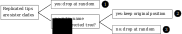
\includegraphics[scale=0.7]{figures/chapter2/chart_phylorep}
\caption[Procedure followed to drop replicated tips from phylogenies]{\textbf{Procedure followed to drop replicated tips from phylogenies.} Most of these were replicated twice, and were sister clades. In that case, tips to drop were chosen randomly, as it did not affect the `true' phylogenetic position of the species (1). When replicated were not sister clades, I kept the tip whose position was closest to the position of the same tip in the uncorrected tree (2). In a few cases, the corrected name did not appear in the original tree. Those were problematic cases, and the tips to drop were chosen randomly (3). Nevertheless, occurences of that third case were rare (see table). See SI for more case examples and more details on the procedure.}
\label{chart_phylorep}
\end{figure}

% Table with number of replicates, number of which were sister clades:
% Number of repliated tips, number that are sister clades, number that are truly pbmatic
% occurences of number of replicates.

\paragraph{Random species attachments.} Some species in the trait datasets were not represented in the phylogenies. When applicable, and to increase representation, these species were attached to their genera in the trees at a random position. Only a small fraction of species that had no initial phylogenetic representation were randomly attached to their genera (Table \ref{random_attachments_phy}).

\begin{table}[h!]
\renewcommand{\baselinestretch}{1}
\renewcommand{\arraystretch}{1.5}
\begin{center}\fontsize{9}{11}\selectfont
\caption[Species representation in phylogenetic trees (corrected taxonomy)]{\textbf{Species representation in phylogenetic trees (corrected taxonomy).} The number of species randomly attached to their genera ranged from 94 (mammals) to 611 (reptiles). Finally, most avian and mammalian species were represented in the phylogenies, whereas more than half reptilian and amphibian species had no known phylogenetic position.} 
\label{random_attachments_phy}
\begin{tabular}{|l|l|l|c|l}
\cline{1-4}
\multicolumn{1}{|c|}{\textbf{Class}} & \multicolumn{1}{c|}{\textbf{Initially not in tree}} & \multicolumn{1}{c|}{\textbf{Randomly attached}} & \textbf{No final representation in tree} &  \\ \cline{1-4}
Amphibians                  & 58\% (4027 of 6888)                           & 13\% (510 of 4027)                     & \textbf{51\%}             &  \\ \cline{1-4}
Birds                       & 18\% (2084 of 11637)                          & 4.8\% (100 of 2084)                    & \textbf{17\%}             &  \\ \cline{1-4}
Mammals                     & 7.4\% (407 of 5502)                           & 23\% (94 of 407)                       & \textbf{5.7\%}            &  \\ \cline{1-4}
Reptiles                    & 62\% (6391 of 10334)                          & 9.6\% (611 of 6391)                    & \textbf{56\%}             &  \\ \cline{1-4}
\end{tabular}
\end{center}
\end{table}

\paragraph{Correcting for taxonomy: conclusions.}
Overall, correcting for taxonomy in phylogenies improved species representation in the trees (Figure \ref{species_rep_phylo}). Maximising the number of species represented in the phylogenies was important for further trait imputations and for estimating the amount of trait phylogenetic signal. For amphibian and reptilian species figuring in PREDICTS only, phylogenetic representation disproportionally increased ( with a minimum representation of 76\% for PREDICTS amphibians). Nevertheless, correcting phylogenetic tip labels generated replicates for a marginal number of tips, which then had to be dropped from the phylogeny. 

\begin{figure}[h!]
\centering
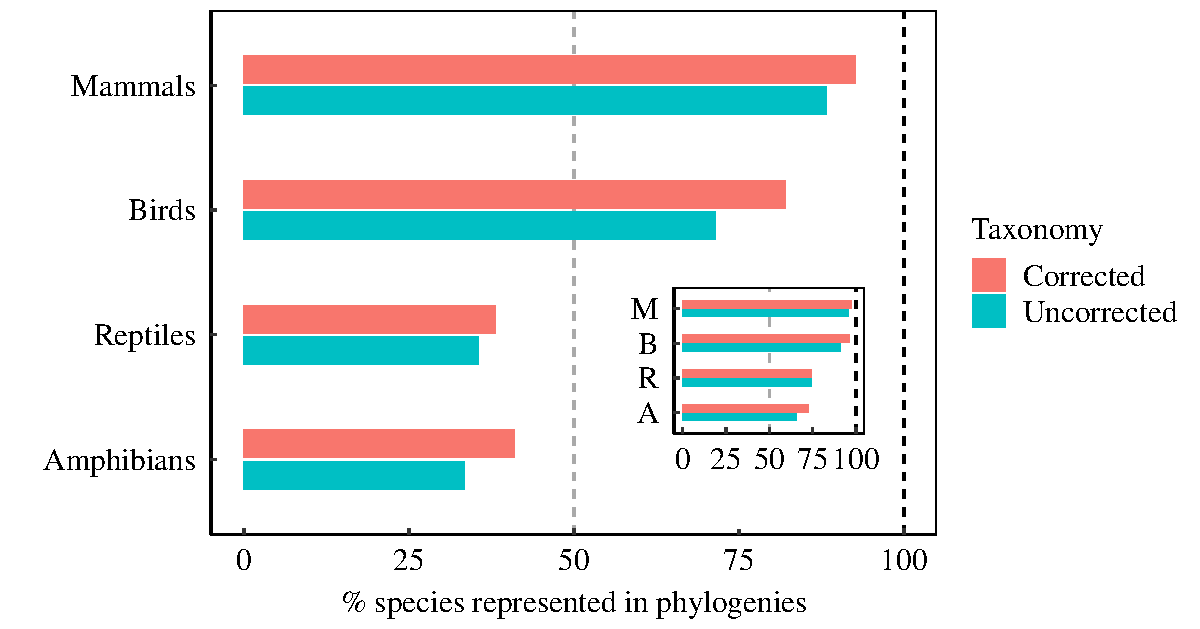
\includegraphics[scale=0.7]{figures/chapter2/Species_representation_phylo}
\caption[Percentage of species represented in the phylogenies for both corrected and uncorrected trait datasets]{\textbf{Percentage of species represented in the phylogenies for both corrected and uncorrected trait datasets.} Overall, taxonomic correction increased species representation in phylogenetic trees. Representation for mammals and birds was high (after taxonomic correction: 83\% of avian and 94\% of mammalian species had a phylogenetic position). On the other hand, reptiles and amphibians were poorly represented (after taxonomic correction: only 44\% of reptilian and 49\% of amphibian species were placed in phylogenetic trees). The inset barplot shows representation for species figuring in PREDICTS. For these, species presence in phylogenetic trees after correction was high across all classes, with a minimum representation of 76\% for amphibians.}
\label{species_rep_phylo}
\end{figure}

Across all classes, correcting for taxonomy increased trait coverage, measured as the percentage of species for which trait information was available (Figure \ref{}).% For mammals and birds, initial trait coverage was high. On the other hand, the variability in coverage was much higher for reptiles and amphibians.

\begin{figure}[h!]
\centering
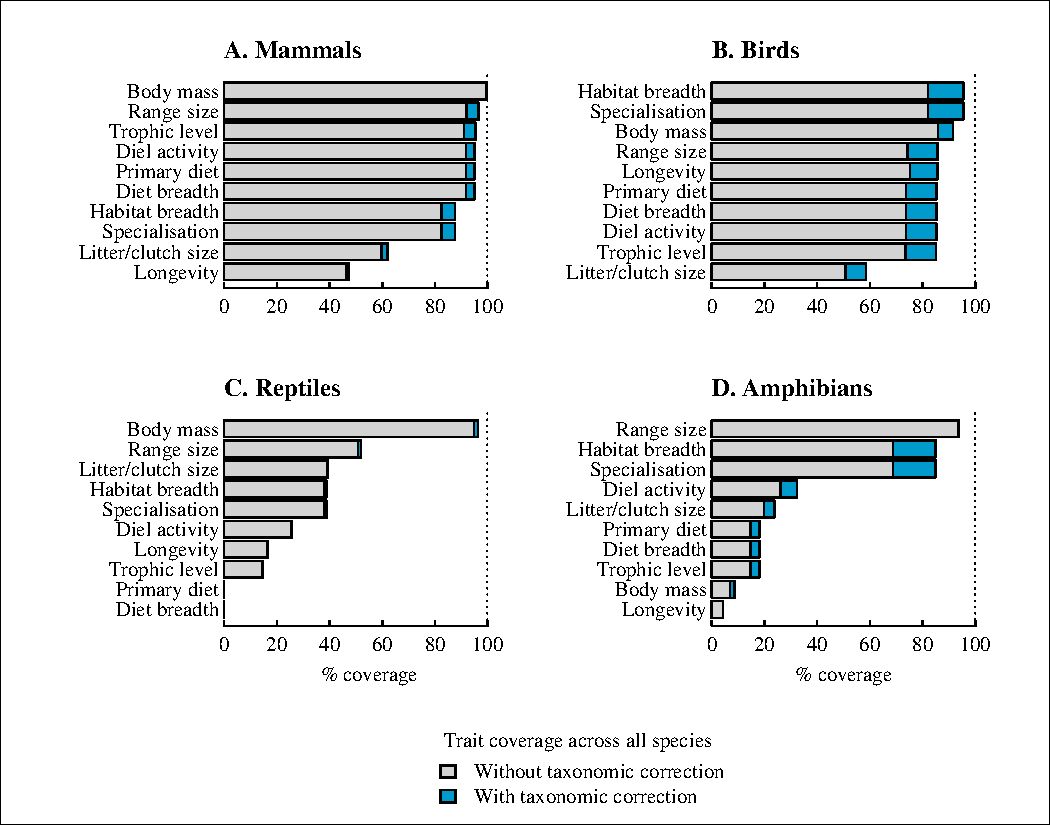
\includegraphics[scale=0.85]{figures/chapter2/Target_traits_All_species_coverage}
\caption[Trait coverage across all species before and after taxonomic correction]{\textbf{Trait coverage across all species before and after taxonomic correction.} Trait coverage is defined here as the percentage of species for which trait information is available. Correcting for taxonomic synonymy improved trait coverage in most cases.}
\end{figure}

For species figuring in PREDICTS, trait coverage disproportionally increased for reptiles and amphibians.

\begin{figure}[h!]
\centering
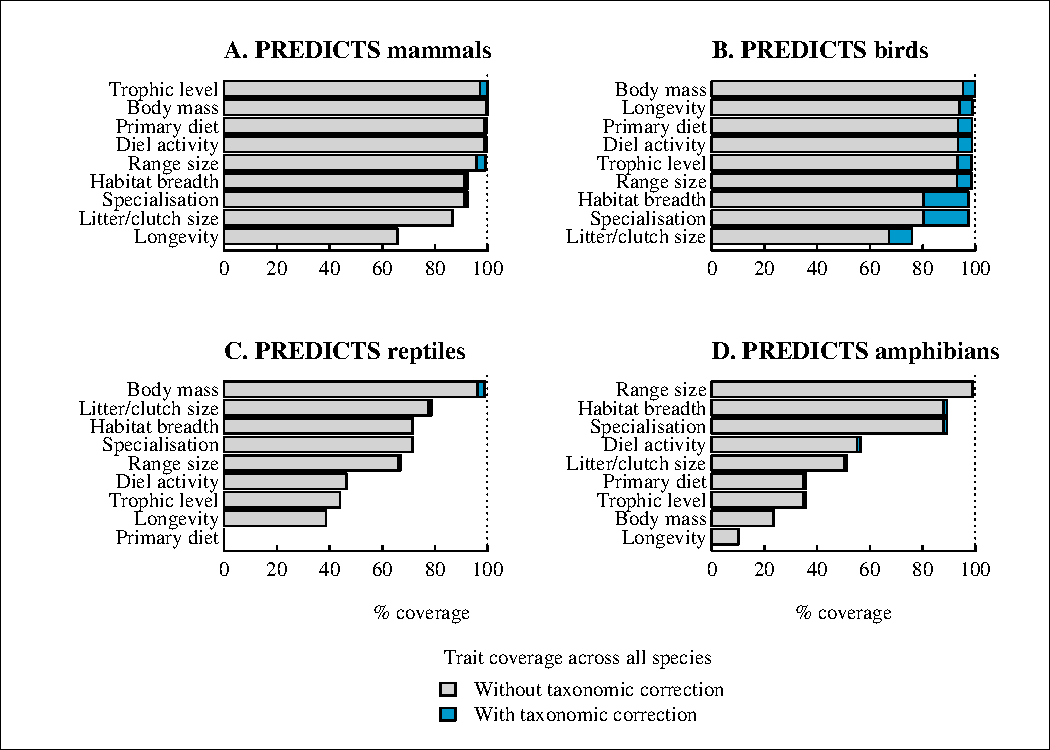
\includegraphics[scale=0.85]{figures/chapter2/Target_traits_Predicts_species_coverage}
\caption[Trait coverage across PREDICTS species before and after taxonomic correction]{\textbf{Trait coverage across all species before and after taxonomic correction.} Trait coverage is defined here as the percentage of species for which trait information is available. Correcting for taxonomic synonymy improved trait coverage in most cases.}
\end{figure}



\subsection{Imputing missing trait values}
Given that coverage was highly variable 


% TODO/
% finir coverage
% Randomness in missing trait values:
% 1) fill information across classes
% 2) randomness missing values <> taxonomy?
% 3)trait phylo signal
% 4) missForest imputations & imputation error / robustness. Compare with Rob's for mammals and birds.

\subsubsection{Randomness in missing trait values}



\subsubsection{Phylogenetic signal}
The phylogenetic signal in all continuous trait was assessed using Pagel's $\lambda$ (phytools package). 

% Please add the following required packages to your document preamble:
% \usepackage{multirow}
\begin{table}[h!]
\renewcommand{\baselinestretch}{1}
\renewcommand{\arraystretch}{1.5}
\begin{center}\fontsize{9}{11}\selectfont
\caption[Phylogenetic signal in continuous traits]{\textbf{Phylogenetic signal in continuous traits and in range size.}} 
\label{physignalcont}
\begin{tabular}{|l|l|l|l|l|l|l|}
\hline
\multicolumn{1}{|c|}{\multirow{2}{*}{\textbf{Pagel's lambda}}} & \multicolumn{6}{c|}{\textbf{Traits}}                                                                                                                                                                            \\ \cline{2-7} 
\multicolumn{1}{|c|}{}                                         & \multicolumn{1}{c|}{\textbf{BM}} & \multicolumn{1}{c|}{\textbf{L}} & \multicolumn{1}{c|}{\textbf{LCS}} & \multicolumn{1}{c|}{\textbf{DB}} & \multicolumn{1}{c|}{\textbf{HB}} & \multicolumn{1}{c|}{\textbf{RS}} \\ \hline
Mammals                                                        & 0.98                             & 0.99                            & 0.99                              & 1.0                              & 0.90                             & 0.99                             \\ \hline
Birds                                                          & x                                & x                               & x                                 & x                                & x                                & x                                \\ \hline
Reptiles                                                       & x                                & x                               & x                                 & x                                & x                                & x                                \\ \hline
Amphibians                                                     & x                                & x                               & x                                 & x                                & x                                & x                                \\ \hline
\end{tabular}
\end{center}
\end{table}

\subsubsection{Imputations of missing trait values}
Penone et al (2014) assessed the performance of four different imputation approaches (K-nearest neighbour (kNN), multivariate imputation by chained equations (mice), random forest algorithms implemented with missForest and phylogenetic imputations implemented with phylopars). They summarised the advantages and disadvantages of each method. Their study showed that the kNN approach resulted in significantly higher imputation errors than the three other approaches. Both missForest and phylopars were the best methods when phylogenetic information was included. Nevertheless, phylopars was much slower than missForest, and could only impute on continuous traits. missForest was faster and could deal with both continuous and categorical data.
% When phylogenetic information was not included, mice was the best method, with fast imputations of both categorical and continuous variables.
Based on these results, I imputed missing trait values using random forest algorithms, as implemented by missForest. Phylogenetic relationships were including by extracting the first 10 phylogenetic eigenvectors for the phylogenies (PVR package Santos 2018) and adding them as predictor variables. Penone et al showed that 10 phylogenetic eigenvectors minimised the imputation error. 

% A certain amount of species did not figure in the phylogenies. Keeping order, family and genus information for these?


Robustness of imputations

\pagebreak
\section{Results}

\subsection{Comparing data collation outputs for mammals and birds}

\subsubsection{Collected traits}

\paragraph{Comparison of initial coverage}
\begin{figure}[h!]
\centering
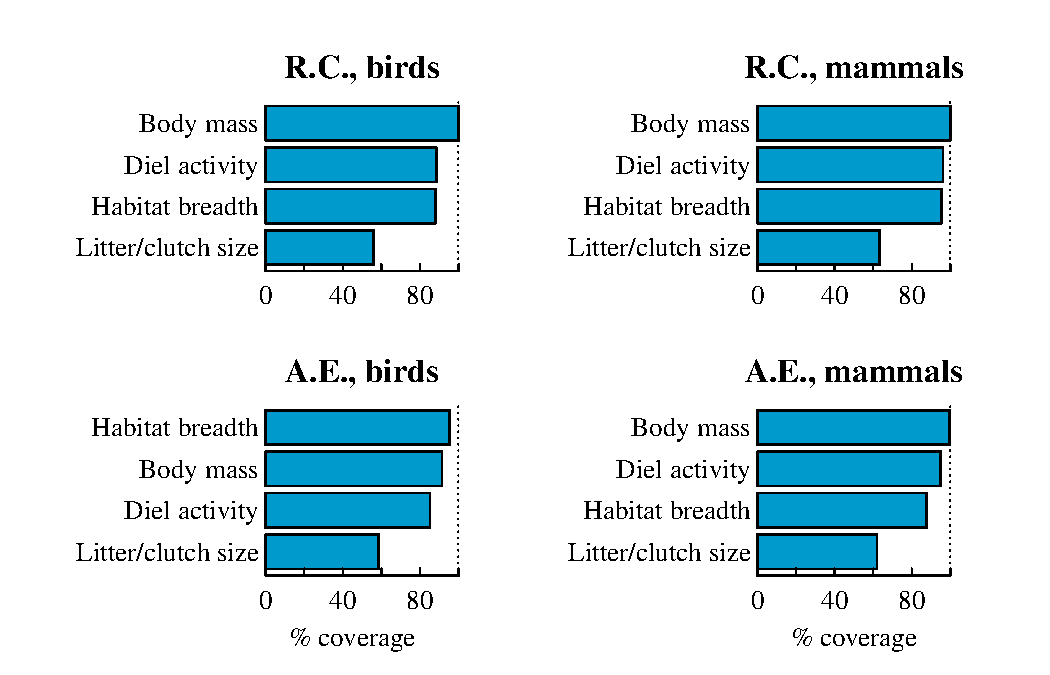
\includegraphics[scale=0.7]{figures/chapter2/Comparison_with_RCooke/Coverage.pdf}
\caption[]{}
\label{ComparisonRC_coverage}
\end{figure}

\paragraph{Comparison of collected trait values}
\begin{figure}[h!]
\centering
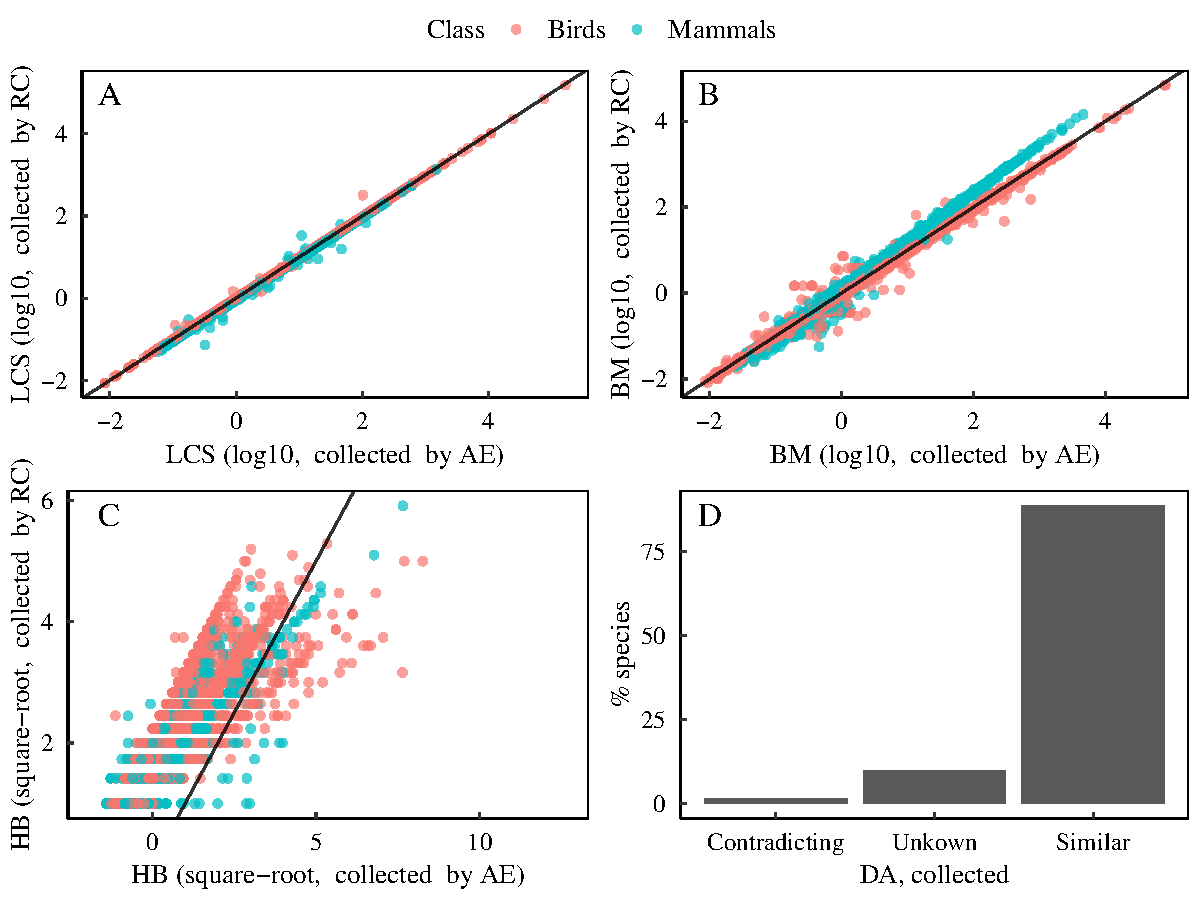
\includegraphics[scale=0.7]{figures/chapter2/Comparison_with_RCooke/Comparison_collected.pdf}
\caption[]{}
\label{ComparisonRC_collected}
\end{figure}

\subsubsection{Imputed traits}
\begin{figure}[h!]
\centering
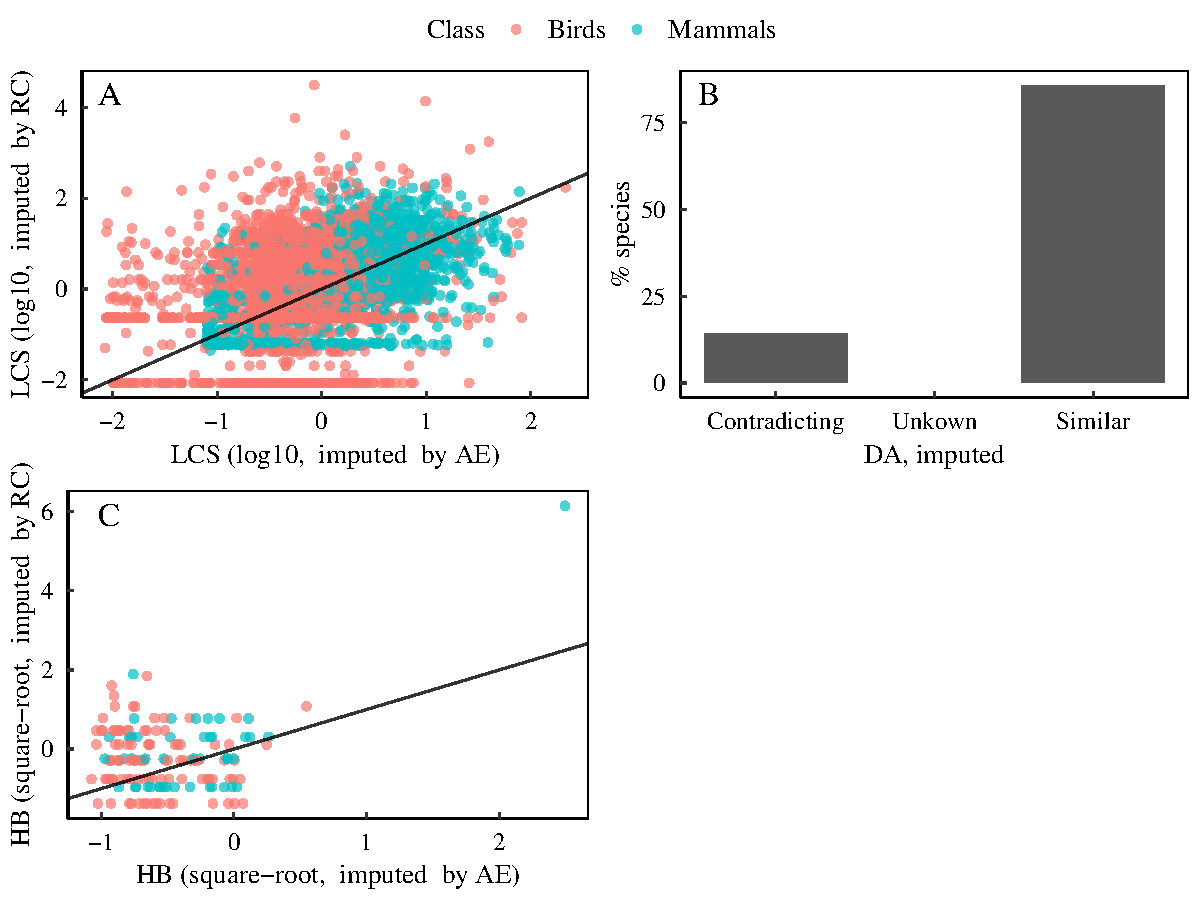
\includegraphics[scale=0.7]{figures/chapter2/Comparison_with_RCooke/Comparison_imputed.pdf}
\caption[]{}
\label{ComparisonRC_imputed}
\end{figure}


\subsubsection{Imputed VS collected}
\begin{figure}[h!]
\centering
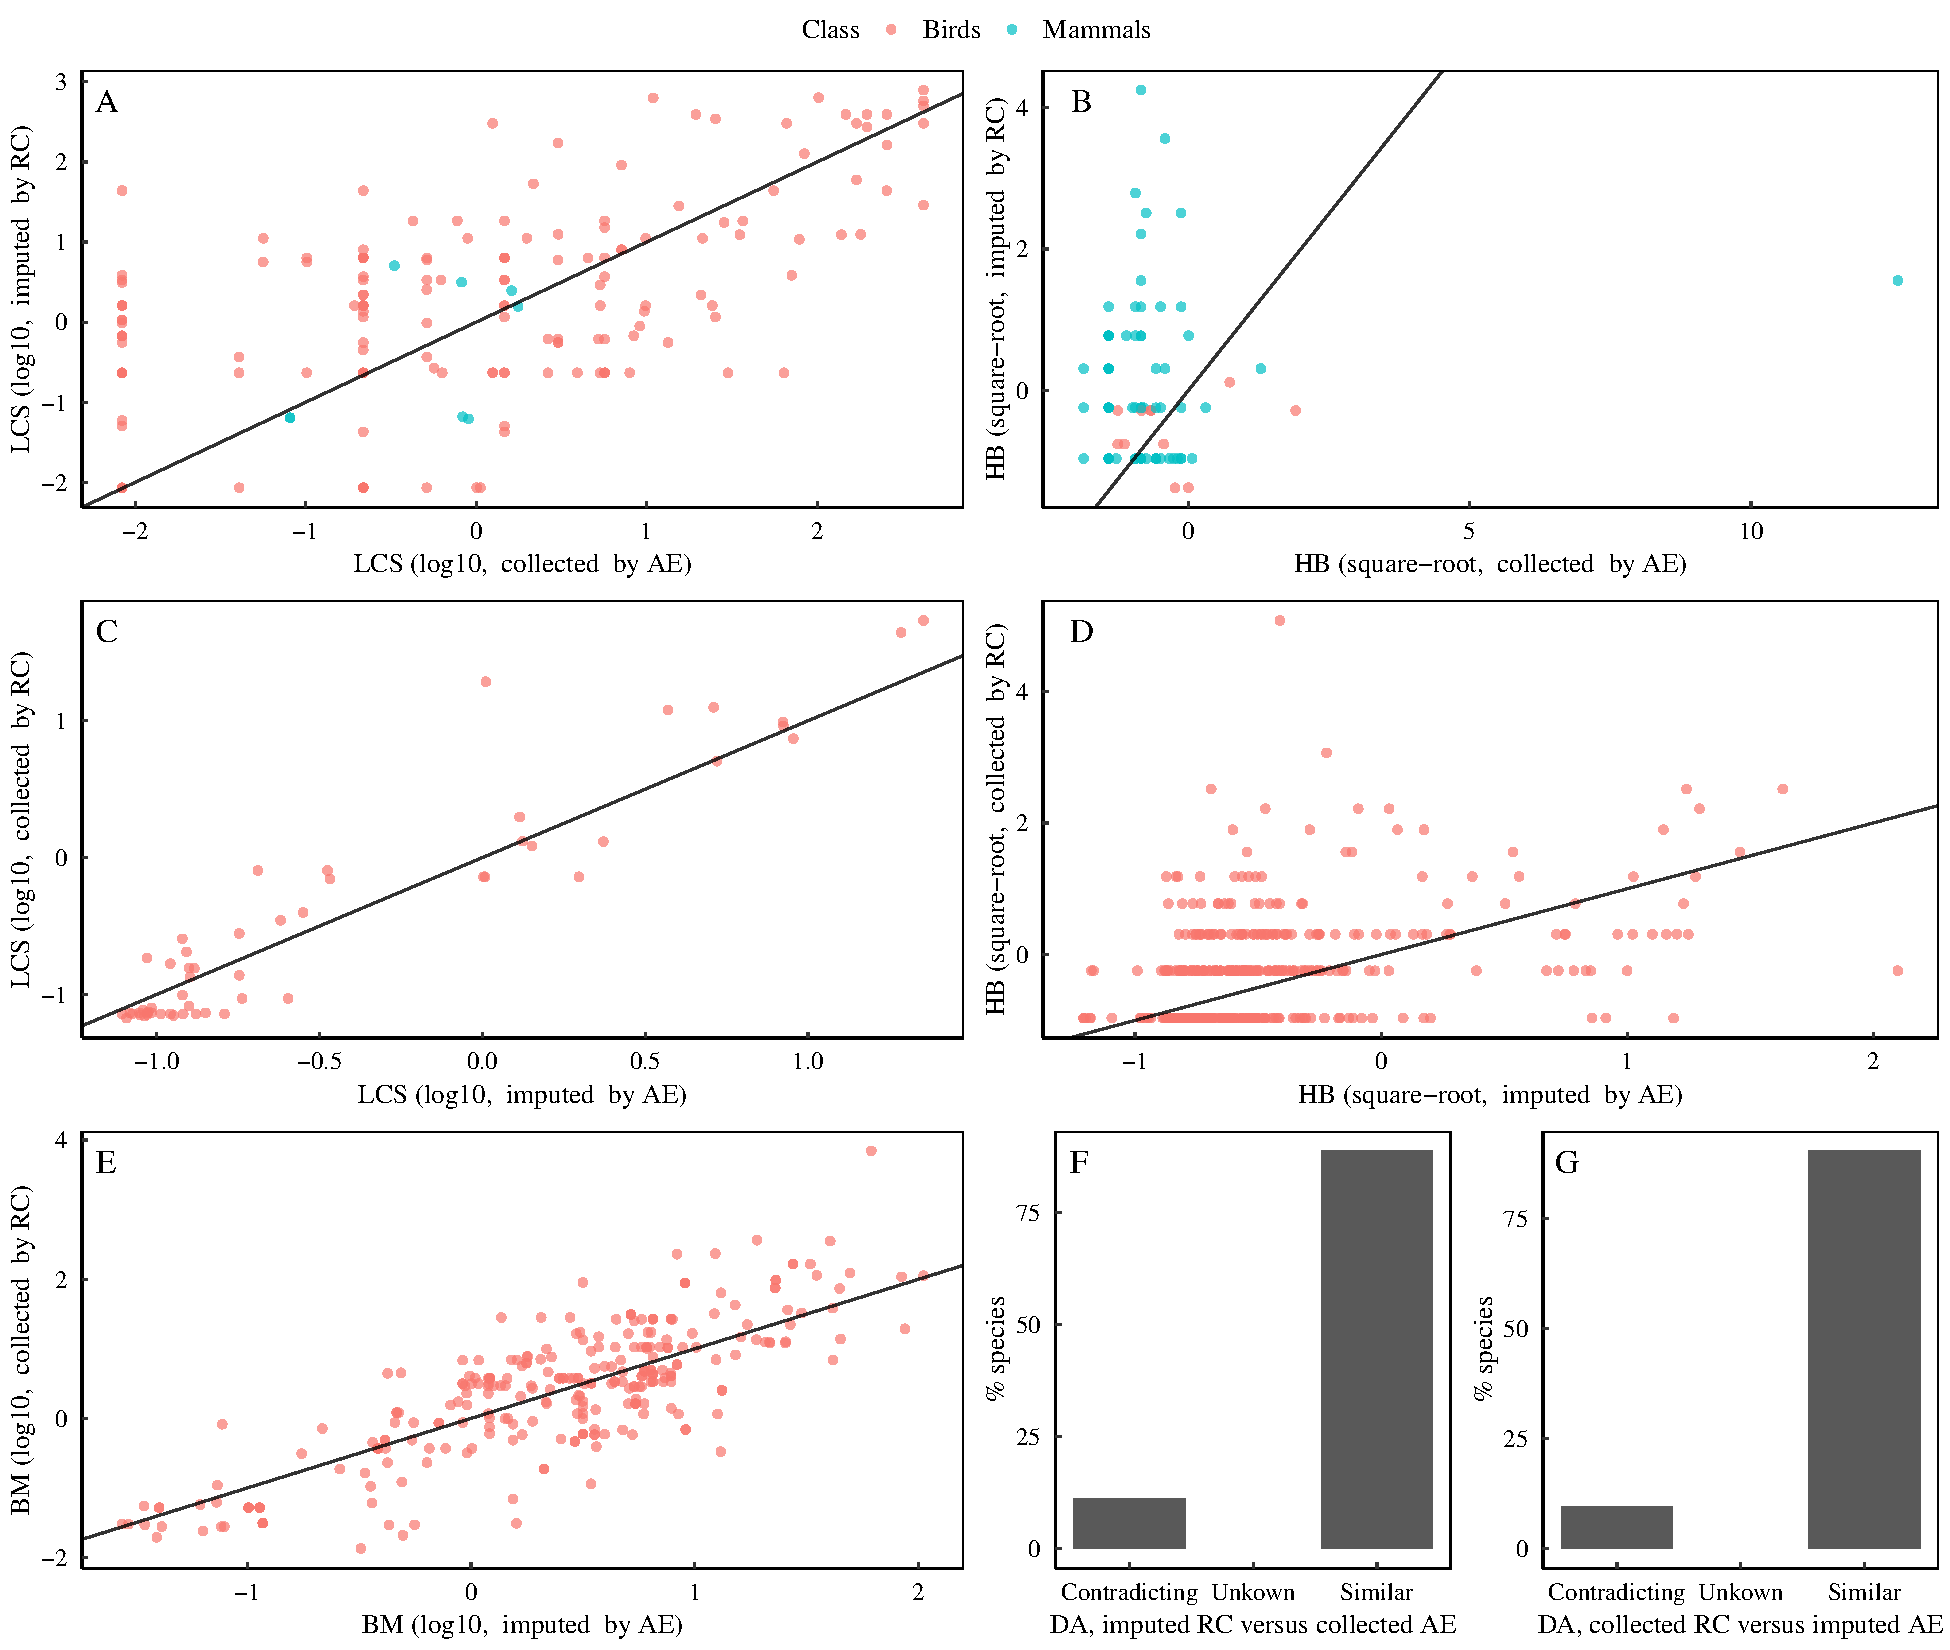
\includegraphics[scale=0.5]{figures/chapter2/Comparison_with_RCooke/Comparison_imputed_VS_collected.pdf}
\caption[]{}
\label{ComparisonRC_VS}
\end{figure}


\subsection{Imputation robustness}

\subsection{Congruence of several imputations}


\section{Discussion}
Discuss taxonomy and robustness of imputations

